\documentclass[polish, 13pt]{beamer}

\usepackage[T1]{fontenc}
\usepackage[polish]{babel}
\usepackage[utf8]{inputenc}
\usepackage[justification=centering]{caption}
\usepackage{subcaption}
\usepackage{booktabs}
\usepackage{array}
\usepackage{amsmath}

% \usetheme{Warsaw}
\usetheme{default}

\title{Zastosowanie autoenkoderów wariacyjnych do rozpoznawania zmian na obrazach medycznych}
\author{Tomasz Nanowski}
\date{15 lutego 2019}
\institute{II UWr}

\AtBeginSection[]{
  \begin{frame}
  \vfill
  \centering
  \begin{beamercolorbox}[sep=8pt,center,shadow=true,rounded=true]{title}
    \usebeamerfont{title}\insertsectionhead\par%
  \end{beamercolorbox}
  \vfill
  \end{frame}
}

\begin{document}

\begin{frame}
\titlepage
\end{frame}

\begin{frame}
\frametitle{Plan prezentacji}
\tableofcontents
\end{frame}

\section{Opis problemu}

\begin{frame}
 \frametitle{Opis problemu}
 \begin{columns}
  \column{0.5\textwidth}
  \textbf{Lokalizowanie zmian nowotworowych} na zdjęciach wykonanych metodą rezonansu magnetycznego (MRI, \textit{ang. magnetic resonance imaging}).
  \column{0.5\textwidth}
  \begin{figure}
    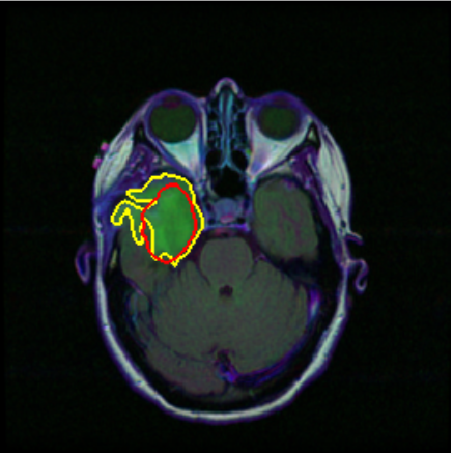
\includegraphics[scale=0.4]{images/MRI}
   \end{figure}
 \end{columns}
\end{frame}

\newcommand\pro{\item[$+$]}
\newcommand\con{\item[$-$]}

\begin{frame}
 \frametitle{Podejście nadzorowane}
 \begin{block}{Opis}
 Bazowanie na danych przeanalizowanych wcześniej przez specjalistów, gdzie każdy przypadek został ręcznie obejrzany i oznaczony. Przykładowo można byłoby skorzystać z architektury \textit{U-Net}.
 \end{block}
 \pause
 \begin{exampleblock}{Zalety}
 \begin{itemize}
    \pro wykorzystanie rzeczywistej wiedzy eksperckiej
 \end{itemize}
 \end{exampleblock}
 \pause
 \begin{alertblock}{Wady}
 \begin{itemize}
    \con zbiór danych kosztowny w przygotowaniu i dalszym rozwoju
    \con ograniczenie do pojedynczego obszaru ciała
 \end{itemize}
 \end{alertblock}
\end{frame}

\begin{frame}
 \frametitle{Podejście wykorzystane w pracy}
 
 \begin{block}{Obserwacja}
  Występujące zmiany nowotworowe są ogólnie rzadkie oraz są pewnym odstępstwem od normy. Można potraktować to jako problem wykrywania obserwacji odstających (\textit{ang. outlier}).
 \end{block}
 \pause
 \begin{block}{Pomysł}
  Wykorzystanie autoenkodera wariacyjnego, który uczy się modelować rozkład prawdopodobieństwa danych treningowych. Próbki mało prawdopodobne będą oznaczane jako patologiczne. 
 \end{block}
 
\end{frame}


\section{Autoenkoder wariacyjny}

\begin{frame}
 \frametitle{Funkcja kosztu}
 \begin{block}{Dolne ograniczenie prawdopodobieństwa}
 \begin{flalign}
 \begin{split}
&\log p (x) \geq -l _ { i } ( \theta , \phi ) = E L B O _ { i } ( \theta , \phi ) = \\ 
&\mathbb { E } q _ { \theta } ( z | x _ { i } ) \left[ \log p _ { \phi } \left( x _ { i } | z \right) \right] - \mathbb { K } \mathbb { L } \left( q _ { \theta } ( z | x _ { i } ) \| p ( z ) \right)
\end{split}
\end{flalign}
\end{block}

Interpretacja:
\begin{itemize}[]
\item $\mathbb { E } q _ { \theta } ( z | x _ { i } ) \left[ \log p _ { \phi } \left( x _ { i } | z \right) \right]$ można utożsamiać z błędem rekonstrukcji, gdyż odpowiada temu składnik $\log p(x|z)$. Dodatkowo jest to potęgowane przez $q(z|x)$, czyli pewność co do reprezentacji ukrytej.

\item $\mathbb { K } \mathbb { L } \left( q _ { \theta } ( z | x _ { i } ) \| p ( z ) \right)$ można interpretować jako ilość przesyłanych informacji, ponieważ jeżeli model będzie chciał odejść od rozkładu a priori $p(z)$ to zapłaci za to karę, ale będzie w stanie przekazać wiadomość.
\end{itemize}
\end{frame}

\begin{frame}
 \begin{figure}
  \centering
  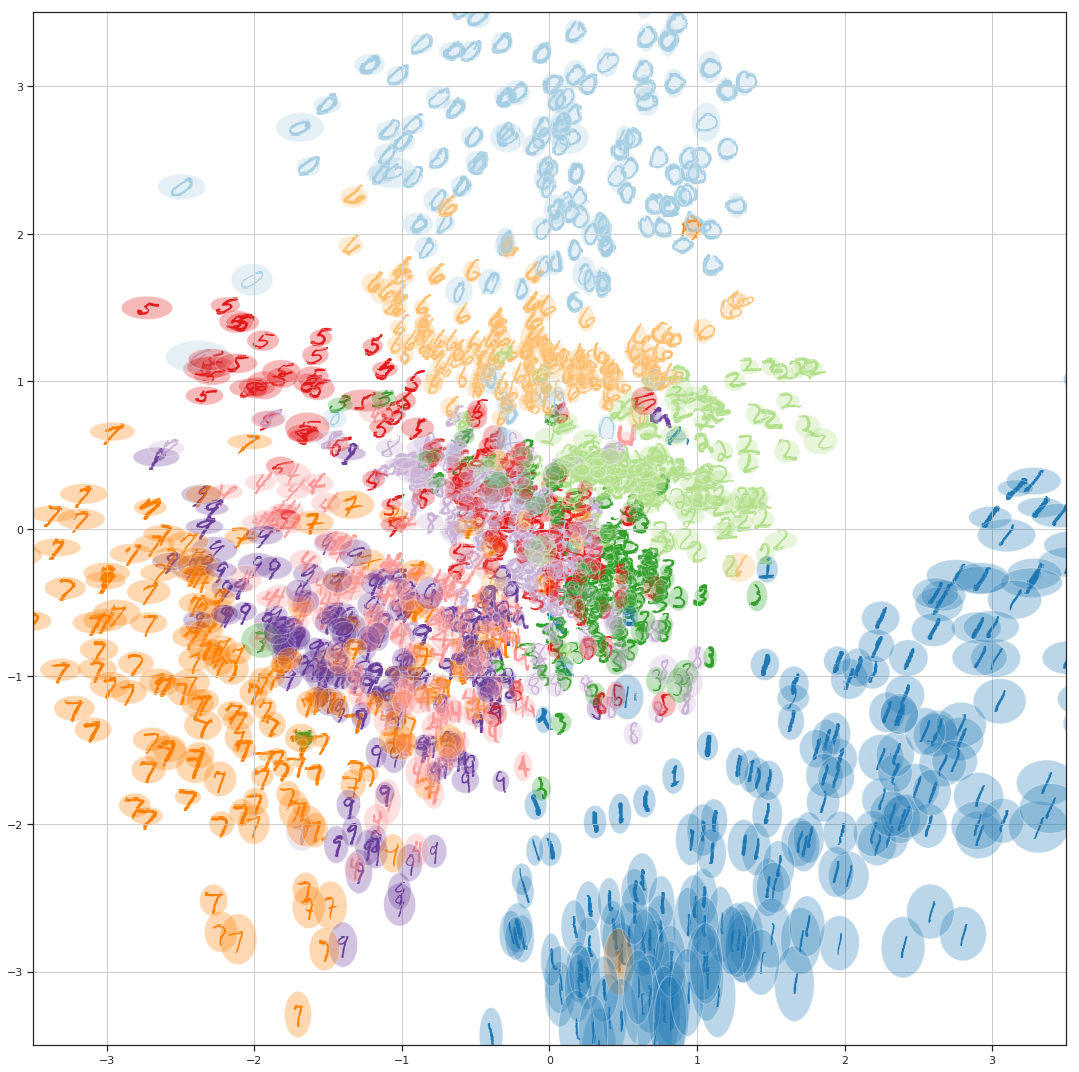
\includegraphics[scale=0.21]{images/mnist_2d}
  \caption{Rozkład konkretnych próbek w przestrzeni ukrytej z zaznaczonym odchyleniem standardowym}
 \end{figure}
\end{frame}

\section{Eksperyment na danych syntetycznych (MNIST)}

\begin{frame}
 \frametitle{Plan eksperymentu}
 Skład zestawu \textbf{uczącego}:
 \begin{itemize}
  \item cyfry \textbf{4, 7} $\sim 99\%$
  \item cyfra \textbf{5} $\sim 1\%$ (próbka odstająca)
 \end{itemize}
 
 \vspace{5mm}
 
 Skład zestawu \textbf{testowego}:
 \begin{itemize}
  \item cyfry \textbf{4, 7} $\sim 50\%$
  \item cyfra \textbf{5} $\sim 50\%$ (próbka odstająca)
 \end{itemize}
 
 \vspace{5mm}
 
 Badałem skuteczność separacji danych na podstawie oszacowania przez model dolnego prawdopodobieństwa $ELBO$ (suma kosztu rekonstrukcji i KLD)
\end{frame}


\begin{frame}
 \begin{figure}
  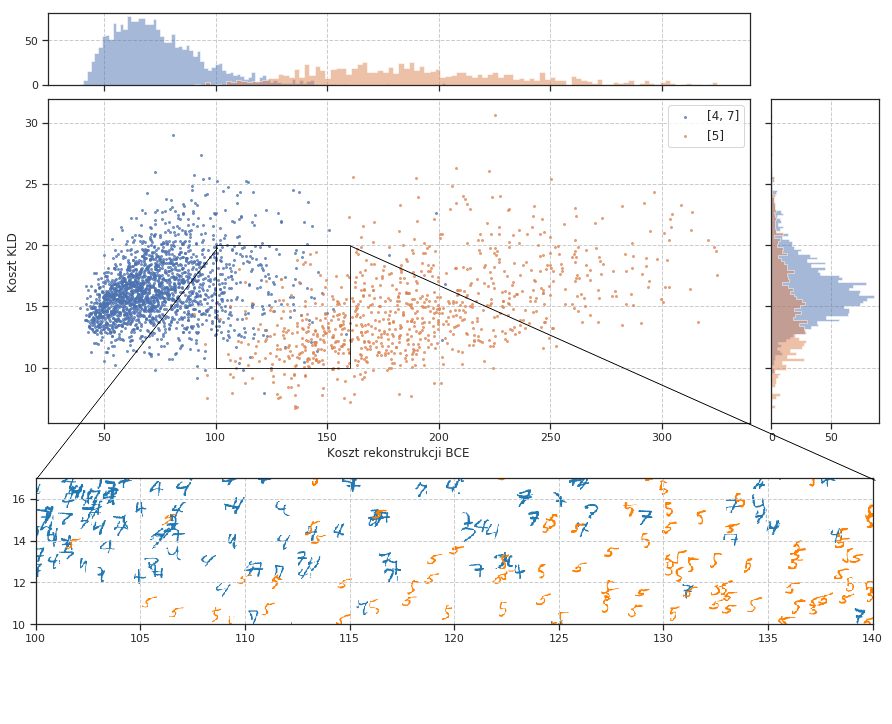
\includegraphics[scale=0.3]{images/mnist_complex}
  \caption{Rozkład próbek wraz z przykładami ze względu na poszczególne składniki funkcji straty}
 \end{figure}
\end{frame}

\begin{frame}
 \begin{figure}
  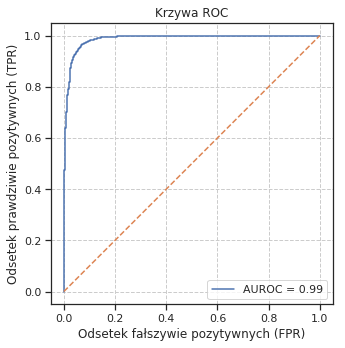
\includegraphics[scale=0.6]{images/mnist_roc_v2}
  \caption{Krzywa ROC dla modelu wyuczonego na danych syntetycznych z zachowaniem odpowiedniej dysproporcji w danych}
 \end{figure}
\end{frame}

\section{Eksperyment na danych medycznych}

\begin{frame}
 \begin{figure}
  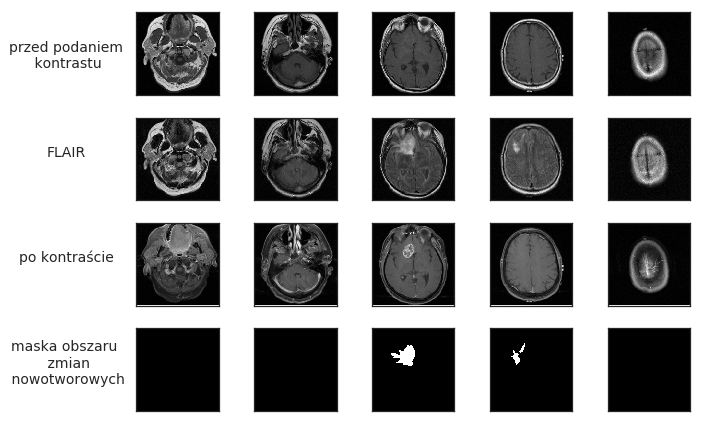
\includegraphics[scale=0.42]{images/medical_description}
  \caption{Przedstawienie konkretnych kanałów w próbce wraz z jego maską zmian}
 \end{figure}
\end{frame}

\begin{frame}
\begin{figure}
  \centering
  \begin{subfigure}[b]{0.45\linewidth}
    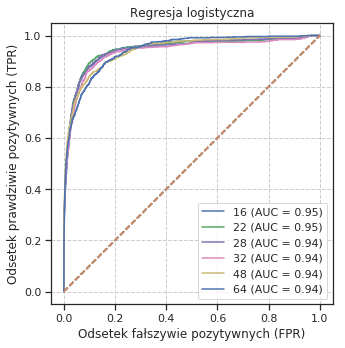
\includegraphics[width=\linewidth]{images/logreg_patch_roc_v2}
    %\caption{}
  \end{subfigure}
  \begin{subfigure}[b]{0.45\linewidth}
    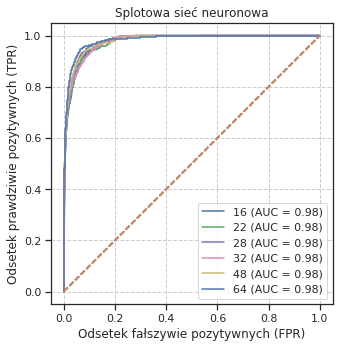
\includegraphics[width=\linewidth]{images/cnn_patch_roc_v2}
    %\caption{}
  \end{subfigure}
  \caption{Porównanie dokładności ze względu na różne rozmiary wycinków dla modeli uczonych metodą nadzorowaną}
  \label{fig:supervised_patches}
\end{figure}
\end{frame}

\begin{frame}
 \frametitle{Wyniki eksperymentu}
 \begin{table}
    \centering
    \begin{tabular}{ l | c c c c c c }
 
    \multicolumn{1}{c}{Model} & \multicolumn{6}{c}{Epoka} \\
    \cmidrule(r){1-1} \cmidrule(r){2-7}
    %\toprule
     		& 1 & 2 & 3 & 20 & 60 & 80 \\ \cmidrule(r){2-7}
    VAE 20-d 	& 0.494 & 0.693 & 0.655 & 0.612 & 0.597 & 0.590 \\ \hline
    VAE 50-d 	& 0.552 & 0.686 & 0.697 & 0.616 & 0.606 & 0.592 \\ \hline
    VAE 100-d 	& 0.580 & 0.685 & \textbf{0.701} & 0.614 & 0.595 & 0.594 \\ \hline
    VAE 200-d   & 0.661 & 0.675 & 0.668 & 0.620 & 0.608 & 0.597 \\ \hline
    VAE 300-d   & 0.704 & 0.671 & 0.657 & 0.620 & 0.600 & 0.593 \\
    \toprule
    \end{tabular}
    \caption{AUC ze względu an rozmiar reprezentacji ukrytej i w różnych stadiach nauki}
\end{table}
\end{frame}

\begin{frame}
 \begin{figure}
    \centering
    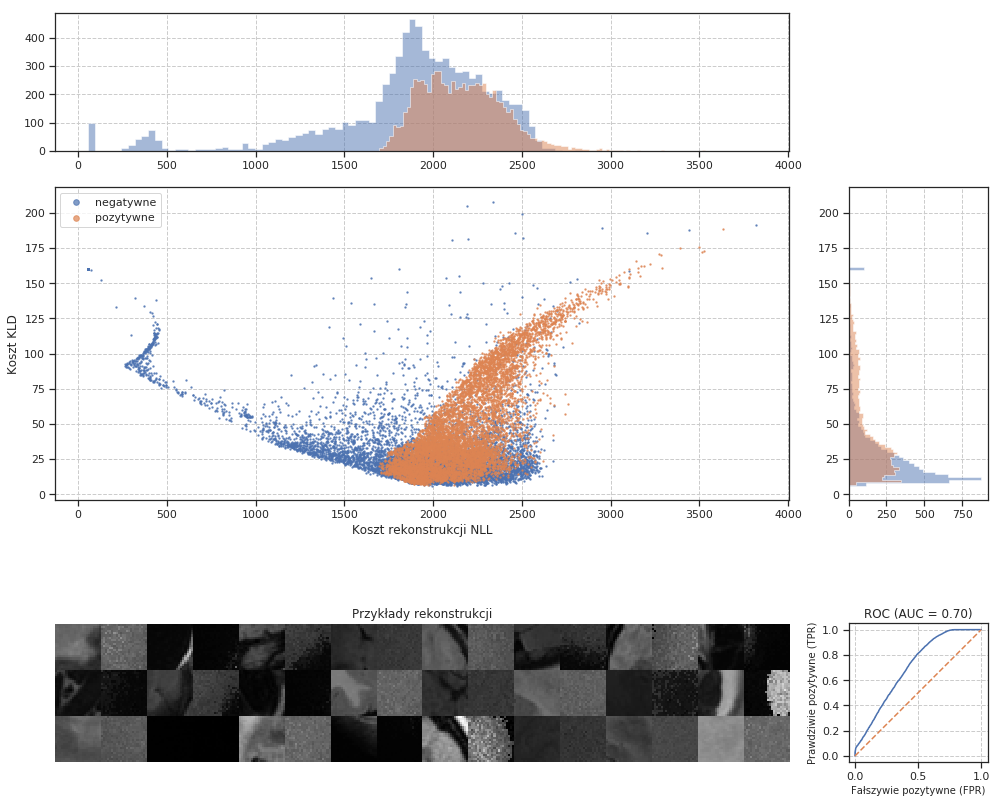
\includegraphics[width=0.9\textwidth]{images/soft_vae_v2}
    \caption{Poszczególne składniki kosztu dla modelu z najlepszą separowalnością}
\end{figure}
\end{frame}

\begin{frame}
\begin{figure}
    \centering
    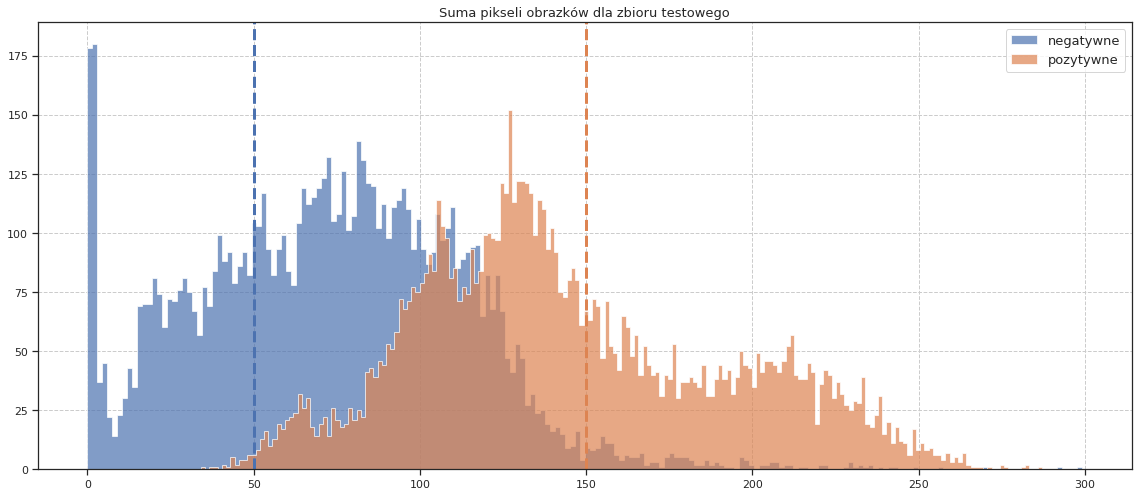
\includegraphics[width=1.0\textwidth]{images/pixels_hist_v3}
    \caption{Rozkład sum pikseli dla obrazków ze zbioru testowego}
\end{figure}
\end{frame}

\begin{frame}
 \begin{figure}
    \centering
    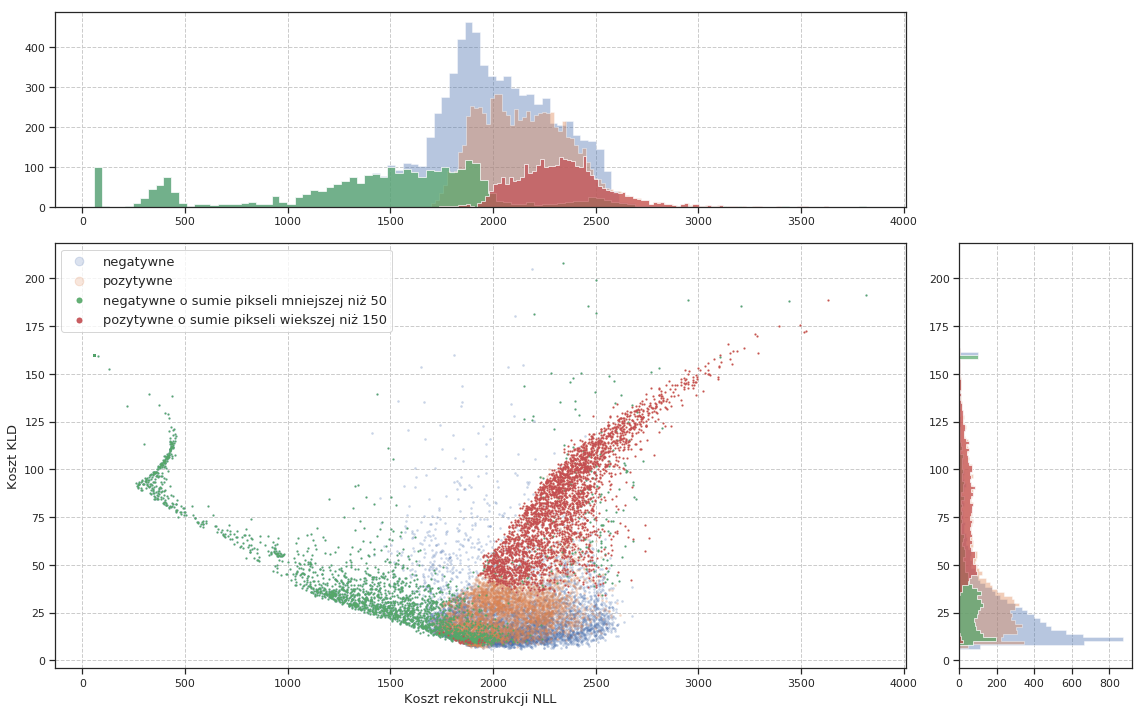
\includegraphics[width=1.0\textwidth]{images/soft_vae_th_v3}
    \caption{Zaznaczenie obrazków o konkretnych sumach pikseli}
    \label{fig:soft_vae_th}
\end{figure}
\end{frame}

\section{Wnioski}

\begin{frame}
 \frametitle{Usprawnienia}
  \begin{itemize}
  \item zastosowanie normalizacji w postaci wyrównywania histogramu (\textit{ang. histogram equalization}), co pozwoliłoby złagodzić jasność
  \item usunięcie zbędnych danych z obrazu w postaci czaszki i oczu, które mogą przeszkadzać w modelowaniu
  \item rozszerzyć kontekst próbki, np. poprzez dodanie dodatkowych informacji o sąsiedztwie do dekodera
 \end{itemize}
\end{frame}


\begin{frame}{}
  \centering \Large
  \emph{Dziękuję za uwagę}
\end{frame}

\end{document}
